% Los sensores integrados del micro:bit — con qué percibe el mundo.
%
% Figura fiel: FOTO REAL del micro:bit (Wikimedia Commons, Gareth Halfacree,
% CC BY-SA 2.0) a la izquierda, y una LEYENDA ordenada a la derecha
% (sensor → qué percibe). El crédito de la foto va en el pie de figura.
% La imagen vive en assets/robotica-1/microbit-foto.jpg (ruta relativa al .tex).
%
% Se incrusta vía \guiaDiagrama desde el bloque `recursos:` del YAML.
\begin{tikzpicture}[font=\sffamily]

  % ── Foto real del micro:bit ──────────────────────────────────────────
  \node[anchor=north west,inner sep=0,draw=milcNegro!20,line width=.4pt]
    (foto) at (0,0)
    {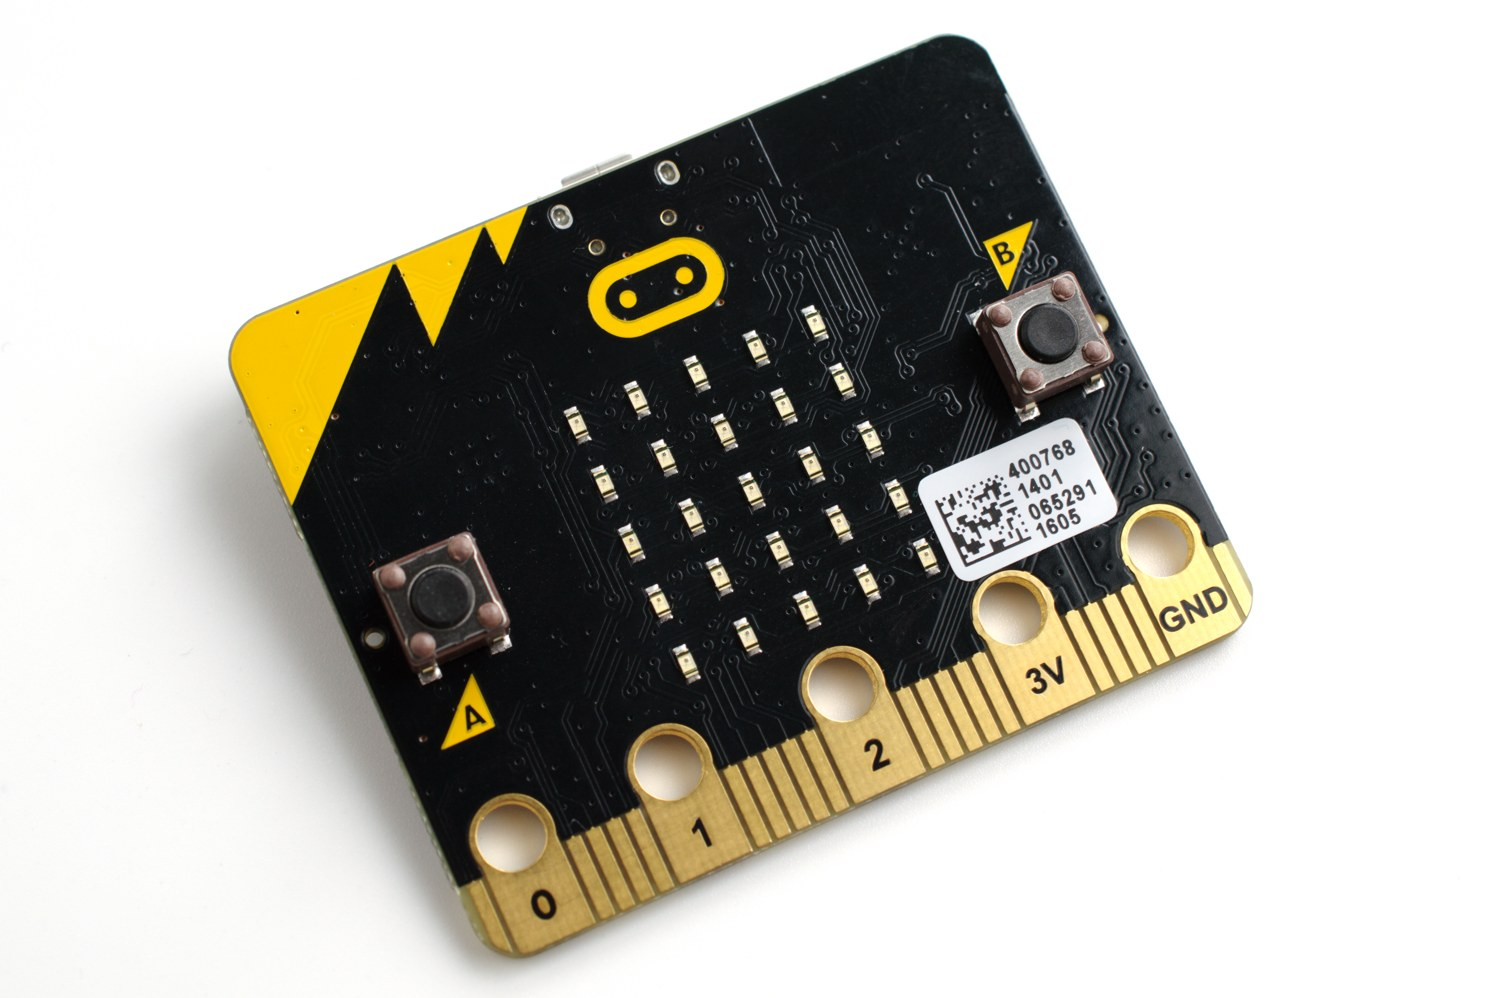
\includegraphics[width=6.5cm]{assets/robotica-1/microbit-foto.jpg}};

  % ── Leyenda: sensor → qué percibe ────────────────────────────────────
  \def\lx{7.0}
  \node[font=\scriptsize\bfseries,milcNegro,anchor=north west] at (\lx,-0.15)
    {Sus «sentidos» vienen adentro (sin cablear):};

  % {y / color-marcador / sensor / qué percibe}
  \foreach \y/\col/\sen/\per in {%
    -0.75/red!85!black/{luz}/{la matriz de LED mide cuánta luz hay}%
    ,-1.30/milcNegro!80/{botones A y B}/{la orden de una persona}%
    ,-1.85/milcTurquesa/{temperatura}/{el calor del ambiente}%
    ,-2.40/milcTurquesa/{acelerómetro}/{movimiento, agitar, caída}%
    ,-2.95/milcTurquesa/{brújula}/{la dirección (campo magnético)}%
    ,-3.50/milcMostaza/{pines (0--GND)}/{tacto y sensores externos}%
  }{
    \fill[\col,rounded corners=1.5pt] (\lx,\y-0.10) rectangle (\lx+0.28,\y+0.16);
    \node[font=\scriptsize\bfseries,milcNegro,anchor=west] at (\lx+0.44,\y+0.03) {\sen};
    \node[font=\scriptsize\itshape,milcNegro!70,anchor=west] at (\lx+2.95,\y+0.03) {\per};
  }

  % ── Moraleja ─────────────────────────────────────────────────────────
  \node[font=\scriptsize\itshape,milcNegro!75,align=center,text width=12cm,anchor=north]
    at (6.0,-4.35)
    {El micro:bit ya trae con qué \textbf{percibir} el mundo, sin cablear nada. La
     pregunta del investigador no es «¿qué sensor tengo?», sino \textbf{«¿qué de mi
     entorno necesita ser percibido?»}.};

\end{tikzpicture}
